\chapter{Related Work}
\label{ch:relatedwork}

In order to tackle the research questions, different disciplines of software engineering such as Complex datasets, Compiler reporting, Continuous integration, Refactoring tools, Issue tracker, Stack Overflow, Gamification, Usability Engineering etc. are looked into and studied what ideas can be adapted into our scenario along with own novel solution ideas. \\ \\

After the literature review in above-mentioned disciplines, here are a few important takeaways in the scope of this Thesis. In the area of 'Complex datasets', current research where Dix et. al. \cite{Dix} talks about more complex grouping and linking of datasets in the context of a user interface of Spreadsheets application. There could be two datasets with fields having similar meaning and fields which are completely different. So, the key takeaway is about design lessons of extensibility of columns for example, 'venues were geocoded to allow spatial graphs' could be related as an example dates in bug reports to some standard format for all tools used and shown on a unified interface. Next, Gaur et. al. \cite{Gaur} speaks about the linear search problem in indexing as it takes more time for large volumes of data. So, different parameters are introduced to decrease computation time. Example: a database with toys is searched linearly for a given query it takes more time than a modified query let's say a toy in red colour and type horse then the search is simplified by looking at two parameters i.e, colour and type. This sparks the idea of grouping bugs as per module, bug type which could ease user in finding a certain bug on an interface.  \\ \\

In the area of 'Compiler reporting', Horning et. al. \cite{horning} mentions the importance of error logging with statistics as to what the compilers are expected to tell the user. It also mentions, the importance of stating what kind of bugs are not found along with bugs found but in reality this questions the scalability. So, the key takeaway is it is ideal to show the number of certain bugs founds in an analysis. Next in the area of 'Refactoring tools', Dustinca \cite{dustinca} talks about how the Refactoring tools are to be built and in user context, it has to overcome the barrier of discoverability which means the difficulty of use. To assist the developer on this issue, they introduced a smart tag in the context of user editor and notifies which parts of the code can be refactored. This emphasizes the importance of 'on-board' phase which plays a key role in Gamification \cite{gamify} discipline. Hayashi et. al. \cite{Hayashi} illustrates the importance of task level commits in order to maintain edit history of refactorings. This gives an idea of which a user does a bug-fix level commit to addressing the traceability scenario. Mealy et. al. \cite{Mealy} mentions about the importance of usability for software refactoring tools and this could perhaps give some basic guidelines similar to knowing Usability Engineering \cite{usability} discipline. \\ \\

In the area of 'Issue tracker', Baysal et. al. \cite{Baysal} mentions reducing the information overload for a developer in using the issue tracker. It is found out in their there is a too much of information they receive which in fact confuses the developer in how to react, example: the developer receive a high number of bugs reported via email and this leads to a situation where the developer ignore the email. They found out some interesting solution ideas such as having a private dashboard for each developer as it becomes easy to react to issues correspond to them. Expressiveness is one other mentioned in their paper which says an example, severity or priority are vague terms to describe a bug. Perhaps, it is ideal to describe the priory as per team decision instead of personal choice.  This signifies in categorising the results as per categories in our unified interface. Next in 'Stack Overflow', in a research paper by Wang et. al. \cite{stack} it is found there are 10934198 questions on a 'User Interface' topic for example. It is quite challenging to go through such a high volume database but nevertheless, the Stack Overflow team has a friendly user interface as shown in the following  \autoref{fig:stackoverflow}. It uses some clean filter techniques like tags for each topic, priority and trending etc. A research by Treude et. al. \cite{Treude.2011} found out that most of the questions (72.30\%) in Stack Overflow have between 2 and 4 tags. This could perhaps ease in filtering/indexing issues. \\ \\

\begin{figure}[hbt!]
	\centering
	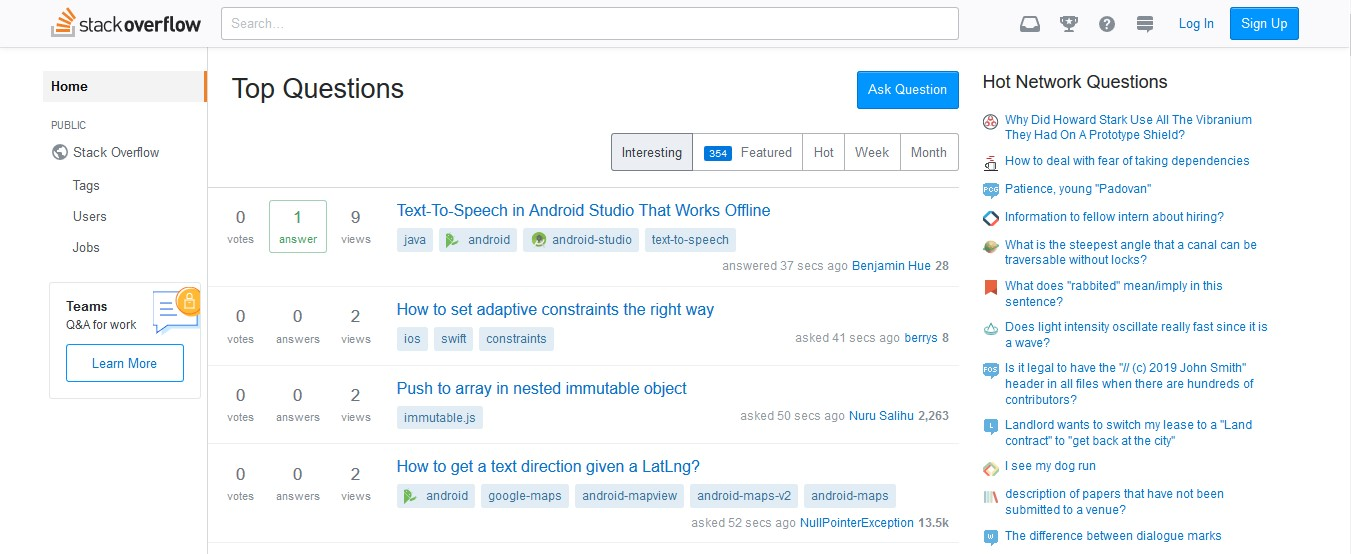
\includegraphics[width=\linewidth]{figures/stackoverflow}
	\caption{An user interface of Stack Overflow Website. \cite{stackoverflow}}
	\label{fig:stackoverflow}
\end{figure}